\documentclass[a4paper]{article}
\usepackage[a4paper, left=1in, right=1in, top=1in, bottom=1in]{geometry}
\usepackage{amsmath}
\usepackage{graphicx}
\usepackage{grffile}
\usepackage{listings}
\usepackage{xcolor}
\usepackage{float}
\usepackage{booktabs}
\usepackage{tikz}
\usepackage{subcaption}
\usepackage{hyperref}
\usepackage{siunitx}
\usepackage{amssymb}

\setlength{\unitlength}{1cm}


\title{MSD: Assignment 2}
\author{Sudhanva Joshi - 2023102022}
\date{15-03-2025}

\begin{document}
\maketitle

\textbf{Note:} Files are hosted on both \href{https://drive.google.com/drive/folders/1z5piVqWysUddM3gHnERhf8o2fc77_pmU?usp=sharing}{Drive} \& \href{https://github.com/sudhu-joshi/msd-a2}{GitHub}.
To run simulations, all file paths must be changed.
\section{CAD Design}
The following dimensions were considered for our links:
\begin{itemize}
    \item Ground Link (L1) = \textbf{150 cm}
    \item Input Link/Crank (L2) = \textbf{75 cm}
    \item Coupler Link (L3) = \textbf{150 cm}
    \item Output Link/Rocker (L4) = \textbf{200 cm}
\end{itemize}
These parameters ensure that \textbf{Grashof's Condition} is satisfied:
\[
S + L \leq P + Q 
\]
\[
L2 + L4 \leq L1 + L3
\]
\[
75 + 200 \leq 150 + 150 
\]

\begin{figure}[H]
    \centering
    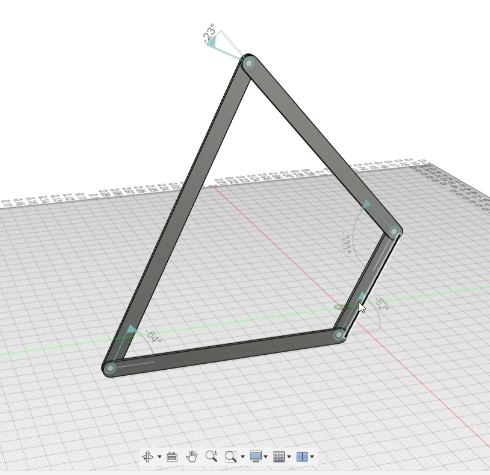
\includegraphics[width=0.6\textwidth]{/home/sudhujoshi/Desktop/Sem_4/MSD/a2/CAD/cad.png}
    \caption{CAD Model of 4-Bar Mechanism}
\end{figure}
\textit{Refer to the video attached for the hitchless $360^\circ$ demonstration.}

\clearpage
\section{Ground Vehicle Data Reconstruction}

\subsubsection*{CSV Data Cleaning}
\begin{itemize}
    \item \textbf{Timestamp Conversion:} 
    \begin{itemize}
        \item The 'timestamp' column is converted to a datetime format using \texttt{pd.to\_datetime}, ensuring compatibility with time-based operations.
        \item Invalid or unparseable timestamps are handled gracefully with \texttt{errors='coerce'}, converting them to \texttt{NaT} (Not a Time) to maintain data integrity.
    \end{itemize}
    \item \textbf{Missing Value Handling:}
    \begin{itemize}
        \item Forward fill (\texttt{ffill}) is applied to propagate the last valid observation forward, ensuring continuity in the dataset.
        \item Backward fill (\texttt{bfill}) is used to fill any remaining missing values with the next valid observation, further enhancing data completeness.
    \end{itemize}
    \item \textbf{Result:} The dataset is cleaned to ensure no missing values, and timestamps are standardized into a consistent, usable format. This process also addresses uneven time intervals, making the data suitable for analysis and reconstruction tasks.
\end{itemize}
Given below are the comparative estimate graphs for both various sensor outputs of both paths.


\begin{figure}[H]
    \centering
    \begin{tabular}{cc}
        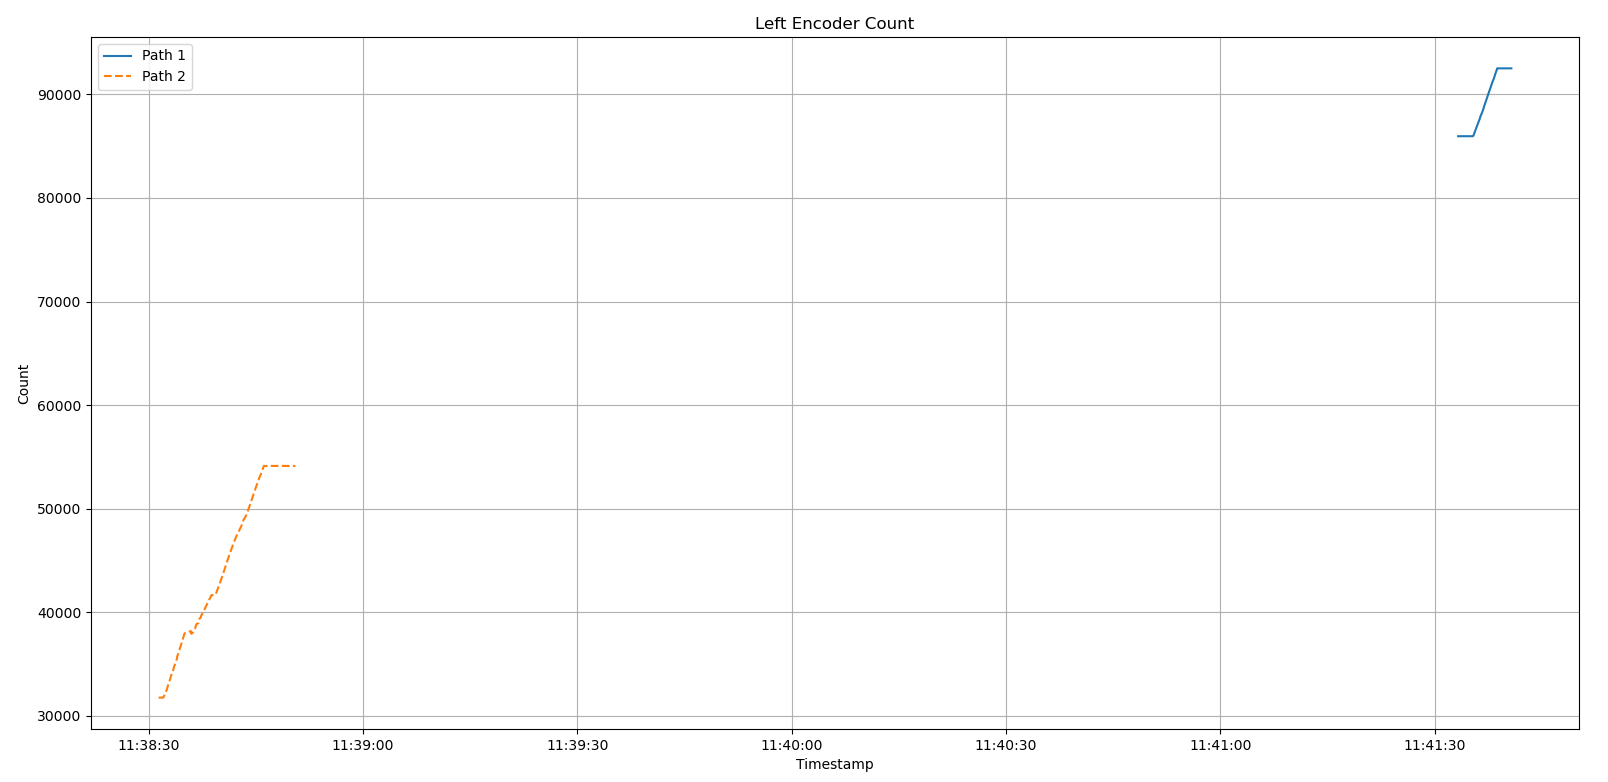
\includegraphics[width=0.45\textwidth]{/home/sudhujoshi/Desktop/Sem_4/MSD/a2/PATH/plots/left_encoder.png} &
        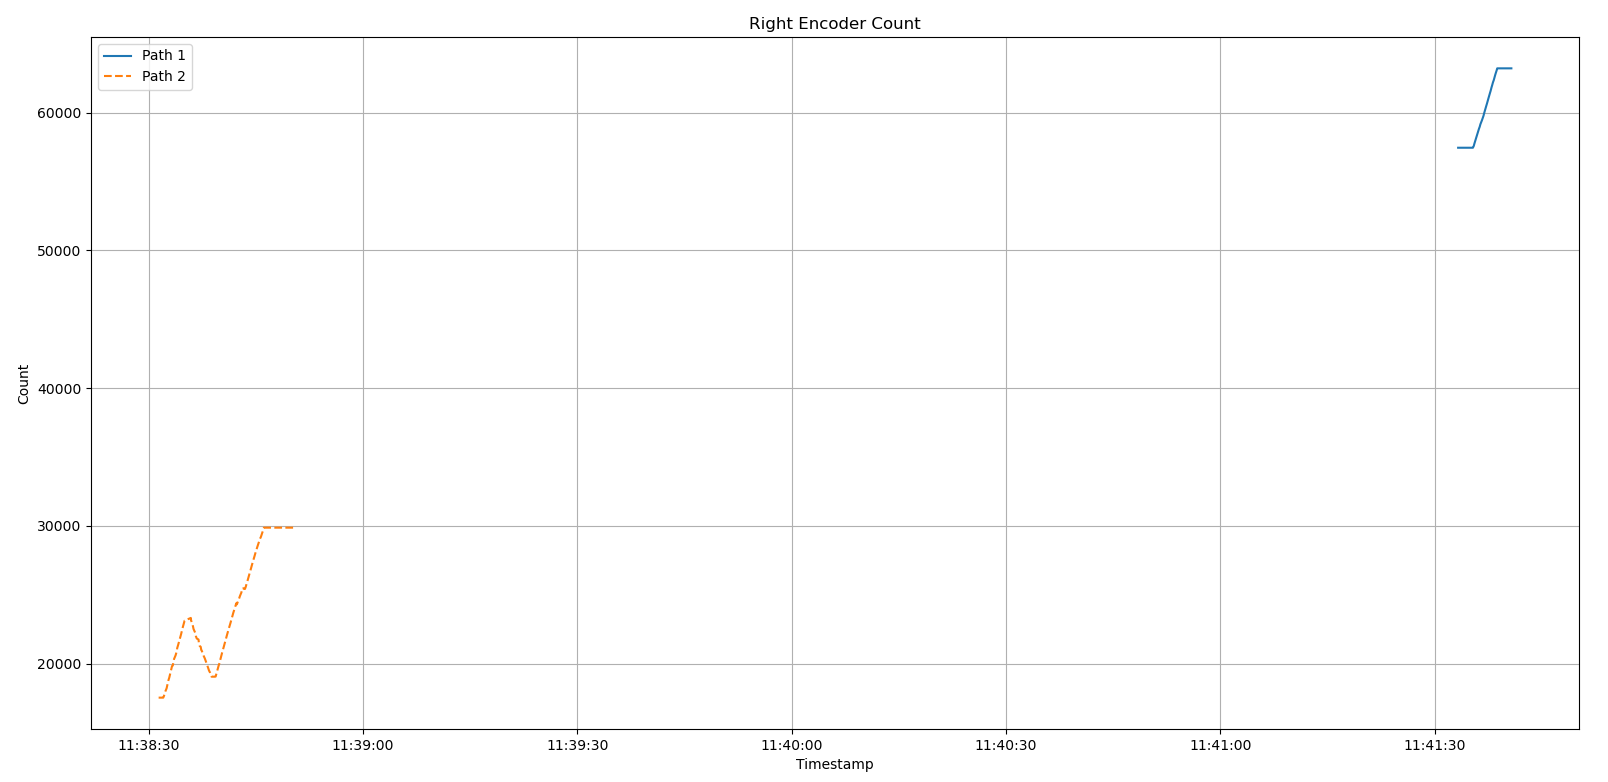
\includegraphics[width=0.45\textwidth]{/home/sudhujoshi/Desktop/Sem_4/MSD/a2/PATH/plots/right_encoder.png} \\
        (a) Left Encoder & (b) Right Encoder \\[10pt]
        
        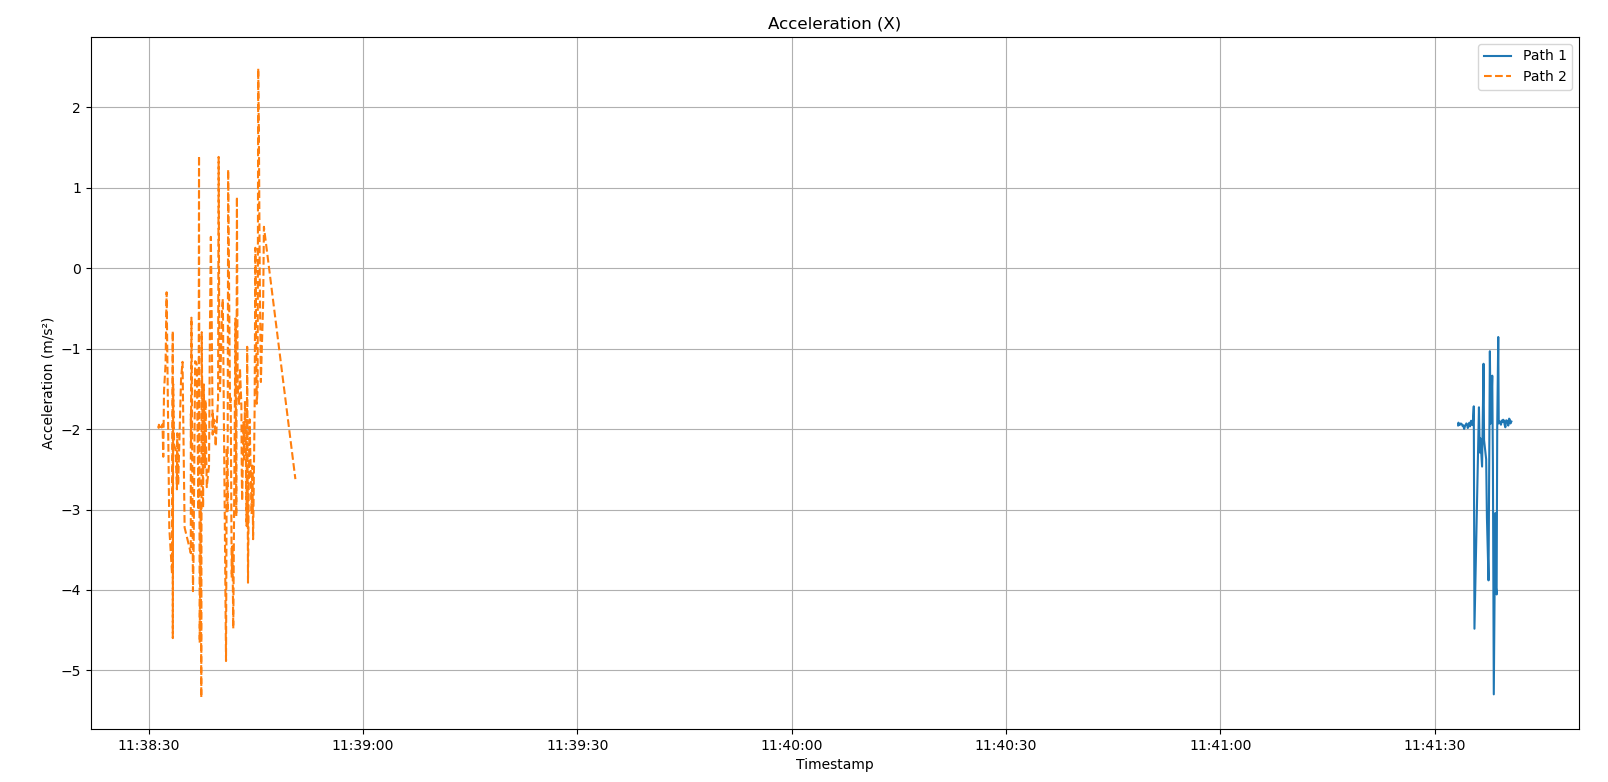
\includegraphics[width=0.45\textwidth]{/home/sudhujoshi/Desktop/Sem_4/MSD/a2/PATH/plots/accelaration.png} &
        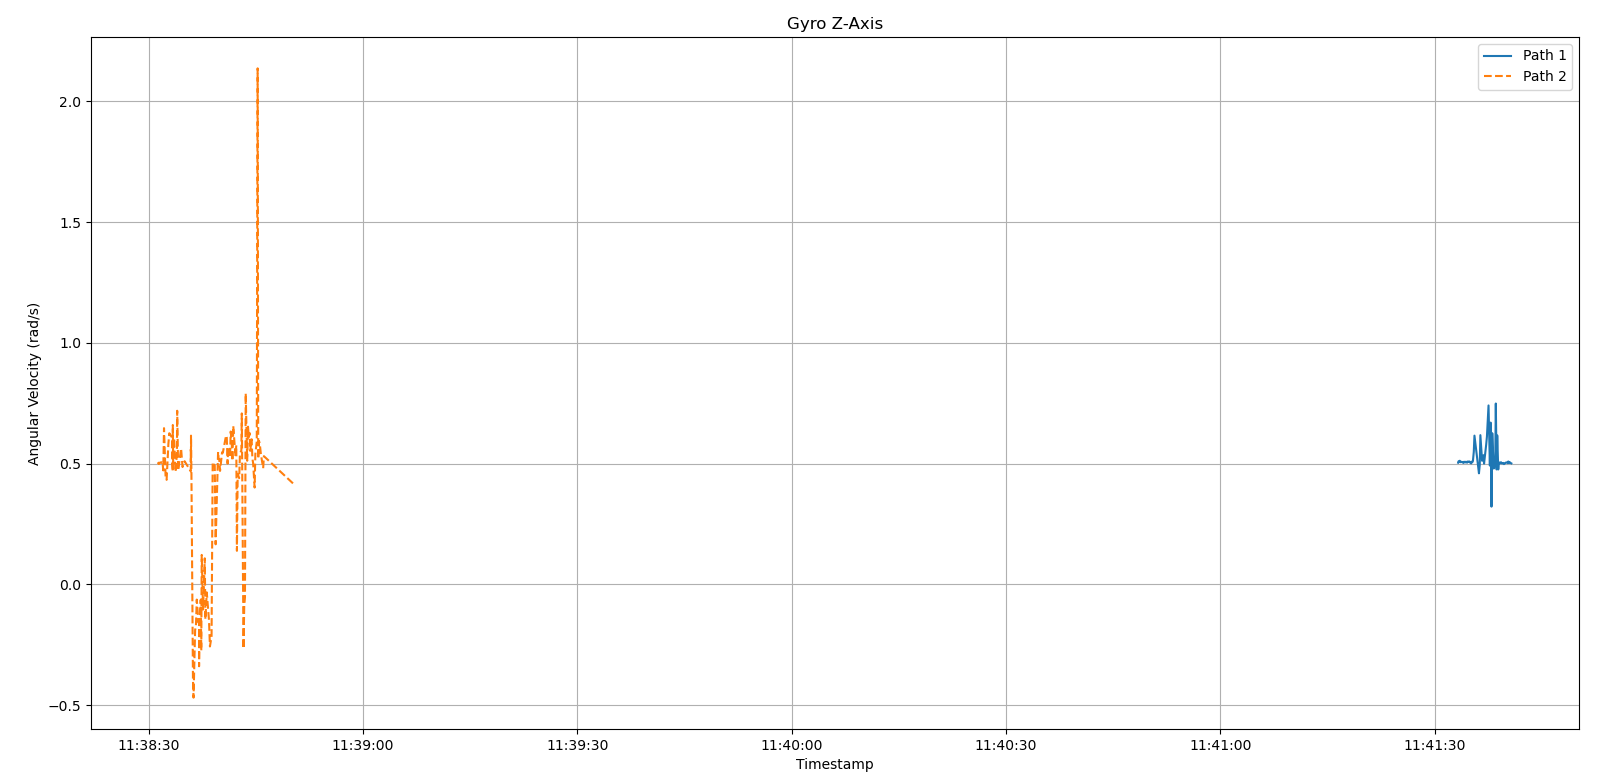
\includegraphics[width=0.45\textwidth]{/home/sudhujoshi/Desktop/Sem_4/MSD/a2/PATH/plots/gyro.png} \\
        (c) Acceleration Reading & (d) Gyro Reading \\[10pt]
        
        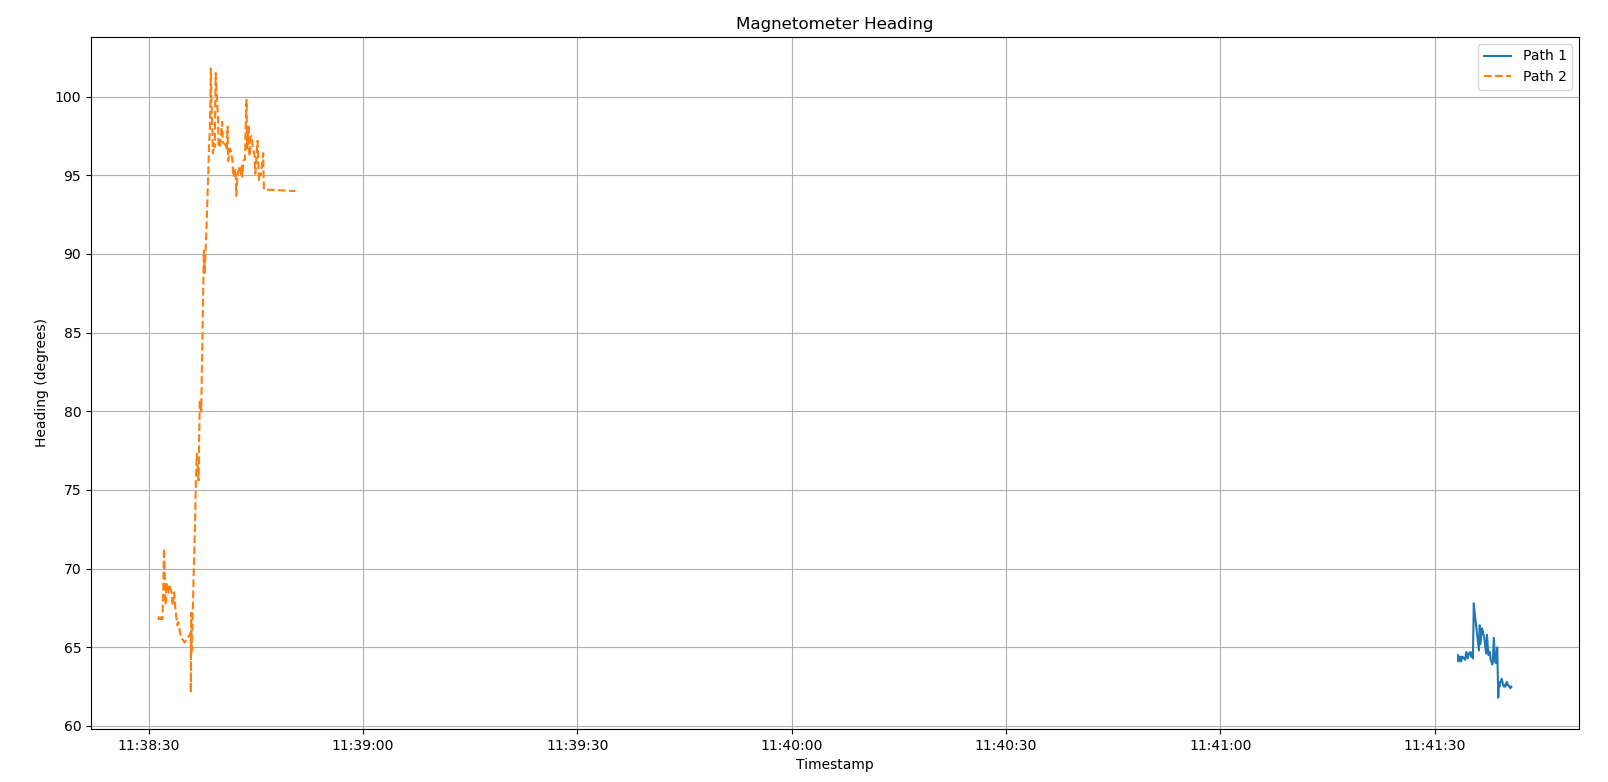
\includegraphics[width=0.45\textwidth]{/home/sudhujoshi/Desktop/Sem_4/MSD/a2/PATH/plots/magnetometer.png} &
        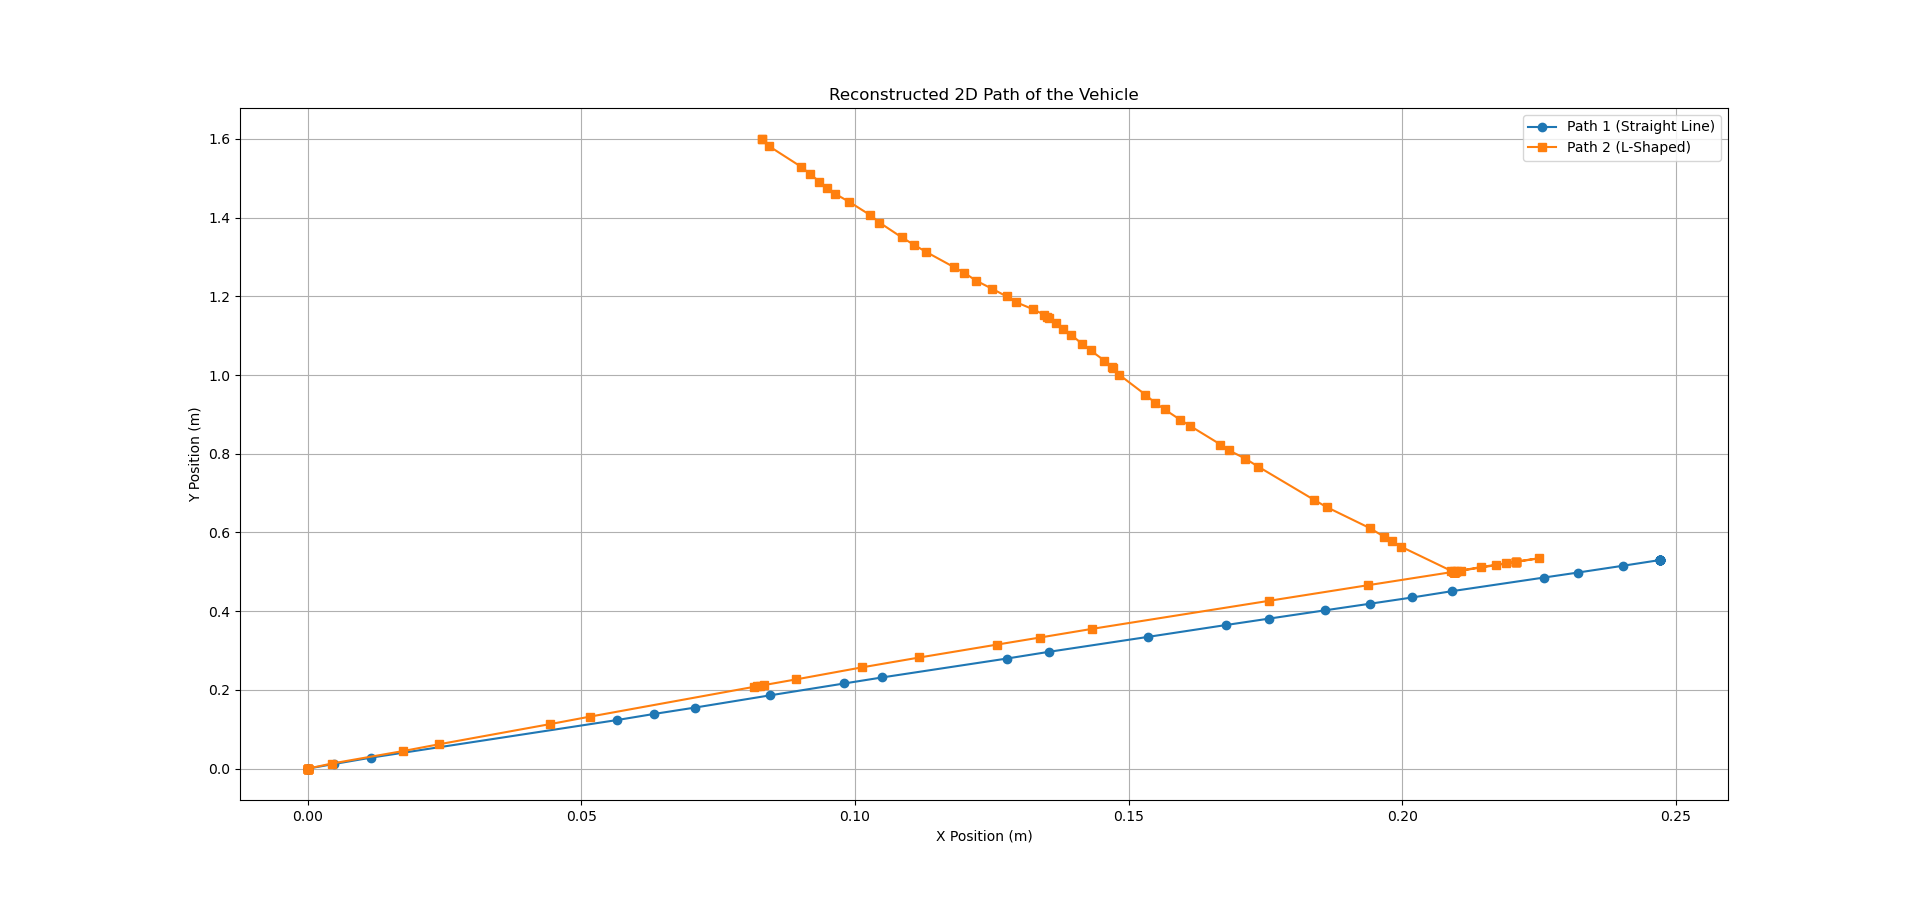
\includegraphics[width=0.525\textwidth]{/home/sudhujoshi/Desktop/Sem_4/MSD/a2/PATH/plots/path_plot.png} \\
        (e) Magnetometer Reading & (f) Cumulative Path Plot \\
    \end{tabular}
    \caption{Sensors \& Reconstructed Data}
\end{figure}


\subsubsection*{Path Reconstruction Process}
The trajectory is reconstructed using encoder and magnetometer data through the following steps:

\begin{itemize}
    \item \textbf{Time Step Calculation:}
    The time difference between consecutive timestamps is computed as:
    \[
    dt = t_i - t_{i-1}
    \]
    where \( t_i \) is the current timestamp and \( t_{i-1} \) is the previous timestamp.

    \item \textbf{Displacement Calculation:}
    The displacement for the left and right tracks is derived from encoder counts:
    \[
    \Delta L = \Delta \text{left\_encoder\_count} \cdot \text{PULSE\_TO\_MM} / 1000
    \]
    \[
    \Delta R = \Delta \text{right\_encoder\_count} \cdot \text{PULSE\_TO\_MM} / 1000
    \]
    where \( \Delta L \) and \( \Delta R \) are the displacements in meters.

    \item \textbf{Orientation Change:}
    The change in orientation (\( \Delta \theta \)) is calculated using the track width (\( W \)):
    \[
    \Delta \theta = \frac{\Delta R - \Delta L}{W}
    \]

    \item \textbf{Heading Integration:}
    The magnetometer heading (\( \theta \)) is used as the primary orientation:
    \[
    \theta = \text{heading} \quad (\text{in radians})
    \]

    \item \textbf{Average Displacement:}
    The average displacement (\( \Delta D \)) is computed as:
    \[
    \Delta D = \frac{\Delta L + \Delta R}{2}
    \]

    \item \textbf{Position Changes:}
    The changes in \( x \) and \( y \) positions are calculated using trigonometry:
    \[
    \Delta x = \Delta D \cdot \cos(\theta)
    \]
    \[
    \Delta y = \Delta D \cdot \sin(\theta)
    \]

    \item \textbf{Cumulative Position:}
    The cumulative \( x \) and \( y \) positions are obtained by integrating the changes:
    \[
    x = \sum \Delta x, \quad y = \sum \Delta y
    \]
\end{itemize}

This process synthesizes encoder and magnetometer data into an approximate 2D trajectory, enabling accurate path reconstruction.

\clearpage
\section{LIDAR, ToF \& Camera Analysis}

\subsection{LIDAR}
\textbf{Note:} To confirm the 2D Point Cloud, the \textit{.pcd} file was visualized using \textit{Blender} as well.
\begin{figure}[H]
    \centering
    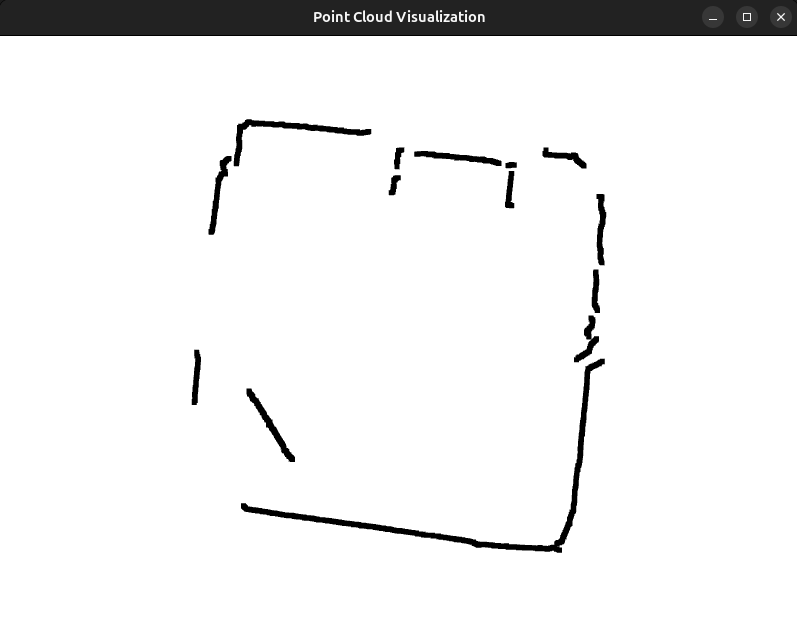
\includegraphics[width=0.6\textwidth]{/home/sudhujoshi/Desktop/Sem_4/MSD/a2/LIDAR/plots/plot.png}
    \caption{2D Point Cloud Form, Open3D} 
\end{figure}
\begin{figure}[H]
    \centering
    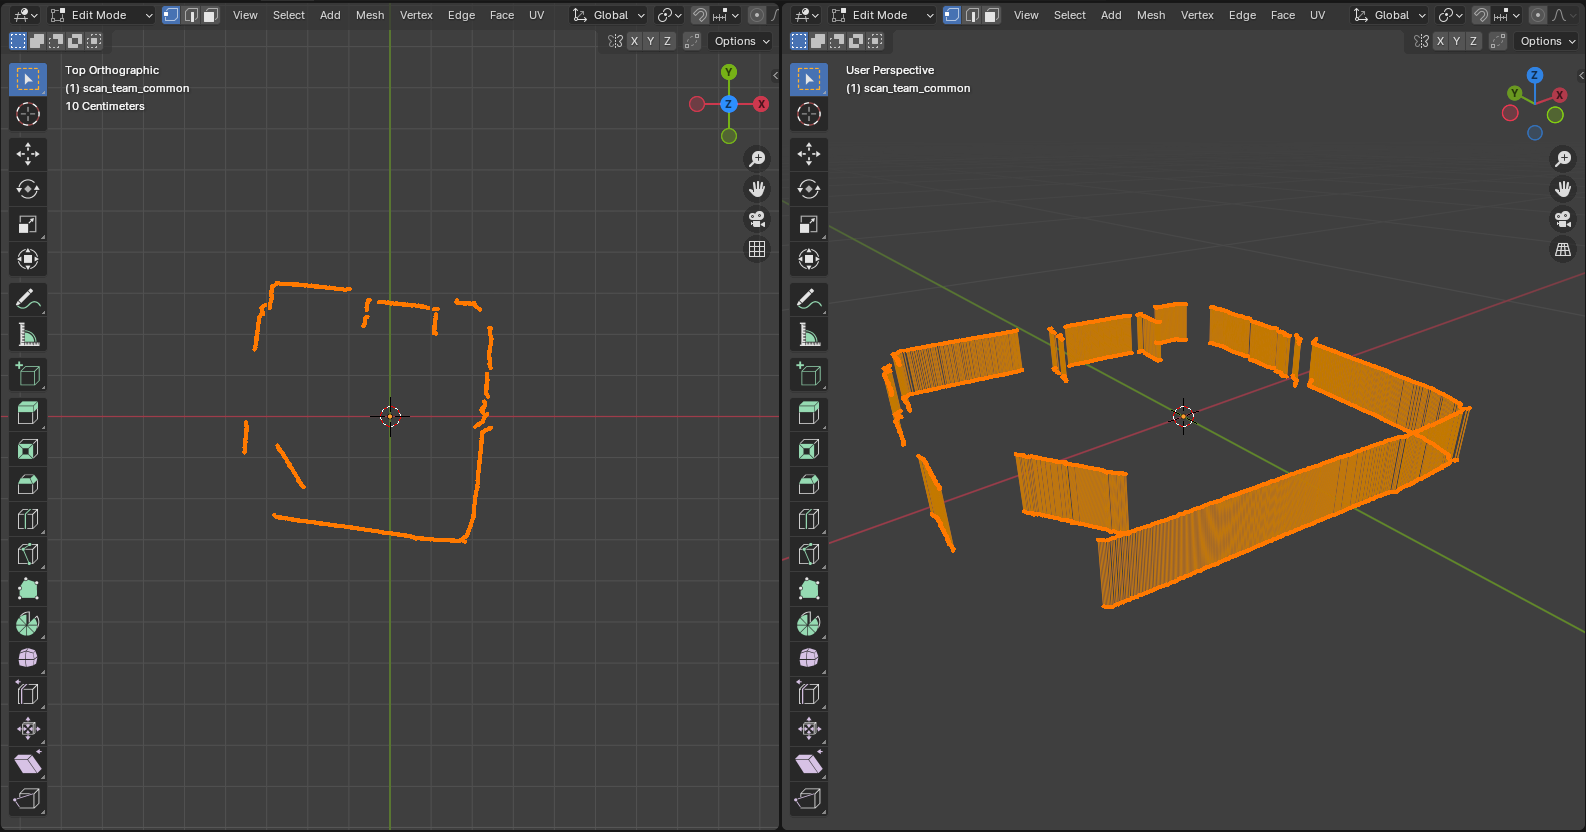
\includegraphics[width=0.65\textwidth]{/home/sudhujoshi/Desktop/Sem_4/MSD/a2/LIDAR/plots/blender_plot.png}
    \caption{Blender Visualization, pcd files imported using \href{https://github.com/MarkHedleyJones/blender-pcd-io/tree/master/io_pcd}{this plugin}}
\end{figure}

\subsubsection*{Detection of Black Objects in 2D LIDAR Point Cloud}
\begin{itemize}
    \item \textbf{Issue:} Black objects are not detected in the plotted LIDAR data.
    \item \textbf{Reason:} Black surfaces have low reflectivity, absorbing most incident light, especially at LIDAR's near-infrared wavelengths (e.g., 905 nm or 1550 nm).
    \item \textbf{Result:} Insufficient reflected signal for detection, leading to missing data points.
    \item \textbf{Contributing Factors:}
    \begin{itemize}
        \item Low reflectivity of black surfaces.
        \item Limited sensitivity of LIDAR sensors to weak or absent reflections.
        \item Potential interference from ambient light or noise.
    \end{itemize}
\end{itemize}

\subsection{ZED Camera}
\subsubsection*{3D Reconstruction from Depth Heatmap}
\begin{itemize}
    \item \textbf{Input:} Depth heatmap (HSV format) and RGB color image.
    \item \textbf{Depth Extraction:} Hue channel of HSV heatmap normalized to depth range \([0.1\,\text{m}, 10\,\text{m}]\):
    \[
    d = \left(1 - \frac{H}{180}\right) \cdot (d_{\text{max}} - d_{\text{min}}) + d_{\text{min}}
    \]
    \item \textbf{3D Point Cloud Generation:} 
    \begin{itemize}
        \item Camera intrinsics (\(f_x, f_y, c_x, c_y\)) map pixel \((u, v)\) to 3D coordinates \((x, y, z)\):
        \[
        x = \frac{(u - c_x) \cdot z}{f_x}, \quad y = \frac{(v - c_y) \cdot z}{f_y}
        \]
        \item RGB color assigned to each 3D point.
    \end{itemize}
    \item \textbf{Output:} .ply file containing 3D point cloud with color.
\end{itemize}

The following results are observed from the 3D reconstruction using both methods:
\begin{figure}[H]
    \centering
    \includegraphics[width=0.6\textwidth]{/home/sudhujoshi/Desktop/Sem_4/MSD/a2/ZEDCAM/reconstructs/depth_lab1.png}
    \caption{Lab 1, Method 1} 
\end{figure}
\begin{figure}[H]
    \centering
    \includegraphics[width=0.6\textwidth]{/home/sudhujoshi/Desktop/Sem_4/MSD/a2/ZEDCAM/reconstructs/depth_lab2.png}
    \caption{Lab 2, Method 1} 
\end{figure}

\begin{figure}[H]
    \centering
    \includegraphics[width=0.6\textwidth]{/home/sudhujoshi/Desktop/Sem_4/MSD/a2/ZEDCAM/reconstructs/heat_lab1.png}
    \caption{Lab 1, Method 2} 
\end{figure}
\begin{figure}[H]
    \centering
    \includegraphics[width=0.6\textwidth]{/home/sudhujoshi/Desktop/Sem_4/MSD/a2/ZEDCAM/reconstructs/heat_lab2.png}
    \caption{Lab 2, Method 2} 
\end{figure}

\subsubsection*{Differences Between Depth Matrix and Heatmap-Based Reconstructions}
\begin{itemize}
    \item \textbf{Method 1 (Depth Matrix):} 
    \begin{itemize}
        \item Directly uses precomputed depth values from a depth matrix.
        \item Higher accuracy as depth values are explicitly provided.
        \item No additional processing or conversion steps required.
    \end{itemize}
    \item \textbf{Method 2 (Heatmap):} 
    \begin{itemize}
        \item Converts a heatmap (HSV) into a depth matrix using hue values.
        \item Introduces potential inaccuracies due to heatmap color-to-depth mapping.
        \item Additional processing step (HSV conversion and normalization) required.
    \end{itemize}
    \item \textbf{Observed Differences:}
    \begin{itemize}
        \item Method 1: Cleaner, more precise point cloud with fewer artifacts.
        \item Method 2: May exhibit noise depending on heatmap interpolation and color-depth mapping.
    \end{itemize}
\end{itemize}

\subsubsection*{Reconstruction Complexity}
\begin{itemize}
    \item \textbf{Lab 1:} Simple scene with fewer objects, uniform lighting, and minimal occlusion, leading to cleaner and more accurate reconstructions.
    \item \textbf{Lab 2:} Complex scene with more objects, varied lighting, and increased occlusion, resulting in noisier and less precise reconstructions.
\end{itemize}

\subsection{Time-of-Flight}
\subsubsection*{Working Principle}

Emits light (e.g., infrared laser) to target. Measures time \( t \) for light to reflect back. Distance \( d \) calculated as:
\[
d = \frac{c \cdot t_{flight}}{2}
\]
where \( c \) = speed of light. 
High accuracy, unaffected by target color/reflectivity. Ideal for short-medium range applications.

\subsubsection*{Possible Reasons for Discrepancies}
\begin{itemize}
    \item \textbf{Sensor Limitations:} Accuracy, resolution, calibration errors, or electronic/thermal noise.
    \item \textbf{Target Properties:} Low reflectivity or uneven surfaces reduce signal strength.
    \item \textbf{Environmental Interference:} Ambient light, temperature, or multipath reflections.
\end{itemize}

\begin{figure}[H]
    \centering
    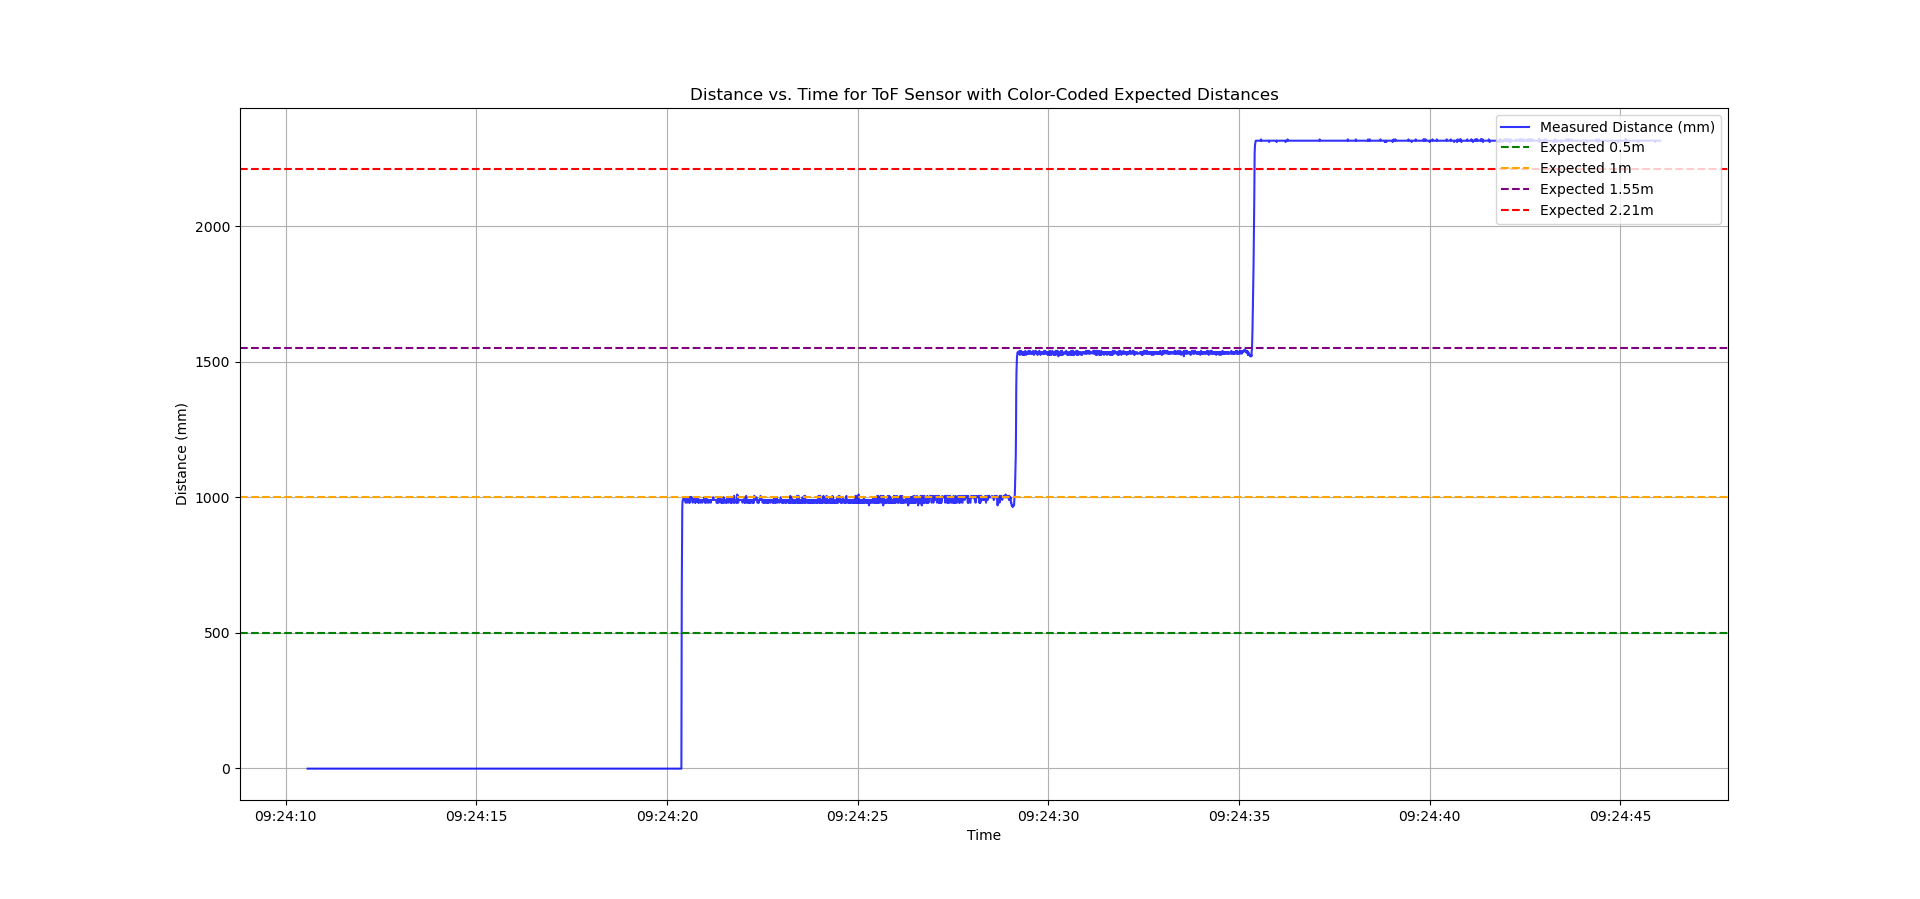
\includegraphics[width=1\textwidth]{/home/sudhujoshi/Desktop/Sem_4/MSD/a2/TOF/tof_distance.png}
    \caption{Estimated Distance vs Time, ToF Sensor} 
\end{figure}





\end{document}

% \begin{figure}[H]
%     \centering
%     \includegraphics[width=0.5\textwidth]{/home/sudhujoshi/Desktop/Sem_4/AEC/Lab/Lab4/imgs/1a.png}
%     \caption{$V_{BE}$ vs $I_{B}$ }
% \end{figure}


% \begin{table}[H]
%     \centering
%     \begin{tabular}{|c|c|c|c|c|c|c|}
%         \hline
%         $V_{BB}$ & $V_{BE}$ & $I_{\beta}$ & $V_{CE}$ & $I_C$ & $\beta=\frac{I_{C}}{I_{\beta}}$ & Region \\
%         \hline
%         0.2V & 0.148V & $5.2 \cdot 10^{-3}$A & 11.95V & $5.0 \cdot 10^{-3}$A & 9.61 & Forward Active \\
%         0.3V & 0.225V & $7.5 \cdot 10^{-3}$A & 11.95V & $5.0 \cdot 10^{-3}$A & 6.66 & Forward Active \\
%         0.4V & 0.328V & $7.2 \cdot 10^{-3}$A & 11.95V & $5.0 \cdot 10^{-3}$A & 6.94 & Forward Active \\
%         0.5V & 0.430V & $7.1 \cdot 10^{-3}$A & 11.95V & $5.0 \cdot 10^{-3}$A & 7.14 & Forward Active \\
%         0.6V & 0.553V & $4.7 \cdot 10^{-3}$A & 11.95V & $5.0 \cdot 10^{-3}$A & 10.6 & Forward Active \\
%         0.7V & 0.618V & $8.2 \cdot 10^{-3}$A & 11.05V & $9.5 \cdot 10^{-3}$A & 115.85 & Forward Active \\
%         0.8V & 0.664V & $1.36 \cdot 10^{-2}$A & 9.35V & $2.65 \cdot 10^{-3}$A & 194.85 & Forward Active \\
%         0.9V & 0.680V & $2.21 \cdot 10^{-2}$A & 7.18V & $4.82 \cdot 10^{-3}$A & 219.09 & Forward Active \\
%         1.0V & 0.700V & $3.0 \cdot 10^{-2}$A & 4.8V & $7.2 \cdot 10^{-3}$A & 240 & Forward Active \\
%         1.2V & 0.720V & $4.81 \cdot 10^{-2}$A & 0.7V & $11.3 \cdot 10^{-3}$A & 235.42 & Saturation \\
%         1.4V & 0.720V & $6.81 \cdot 10^{-2}$A & 0.325V & $11.67 \cdot 10^{-3}$A & 171.62 & Saturation \\
%         1.6V & 0.720V & $8.81 \cdot 10^{-2}$A & 0.2V & $11.8 \cdot 10^{-3}$A & 134.09 & Saturation \\
%         1.8V & 0.720V & $1.081 \cdot 10^{-1}$A & 0.2V & $11.8 \cdot 10^{-3}$A & 109.24 & Saturation \\
%         2.0V & 0.720V & $1.281 \cdot 10^{-1}$A & 0.2V & $11.8 \cdot 10^{-3}$A & 92.18 & Saturation \\
%         3.0V & 0.720V & $2.281 \cdot 10^{-1}$A & 0.2V & $11.8 \cdot 10^{-3}$A & 51.75 & Saturation \\
%         4.0V & 0.720V & $3.281 \cdot 10^{-1}$A & 0.2V & $11.8 \cdot 10^{-3}$A & 35.97 & Saturation \\
%         \hline
%     \end{tabular}
%     \caption{BJT Characteristics}
% \end{table}

